\nxsection{Les Comptes Fournisseurs}
\index{les comptes fournisseurs}

\nxsubsection{Afficher les d\'etails d'un compte fournisseur}
\index{afficher les d\'etails d'un compte fournisseur}
\index{d\'etails d'un compte fournisseur}

\begin{figure}[!htpb]
	\centering
	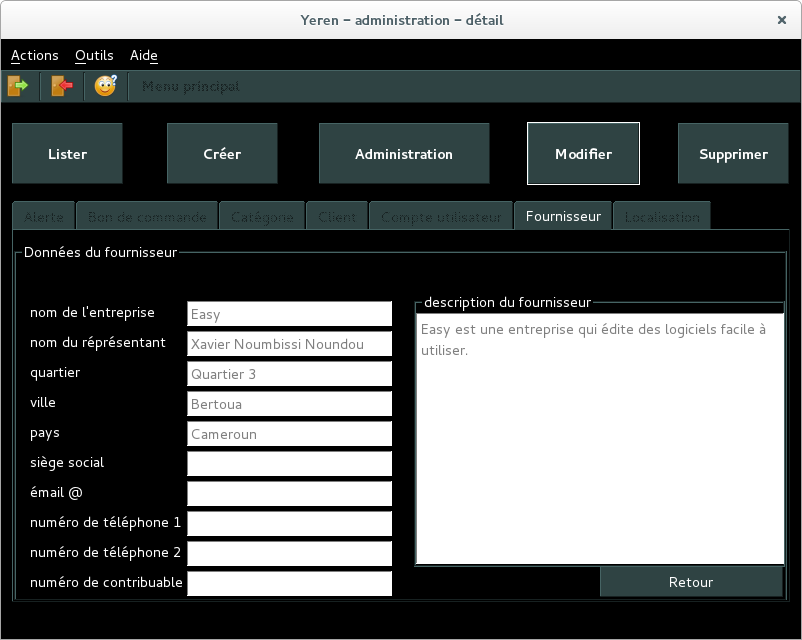
\includegraphics[scale=0.45]{images/compte-fournisseur-afficher-details.png}
	\caption{L'interface graphique pour afficher les d\'etails
			d'un compte fournisseur.}
	\label{fig:admin-fournisseurs-afficher-details}
\end{figure}

La figure~\ref{fig:admin-fournisseurs-afficher-details}
illustre l'interface graphique de \yeren qui affiche
les d\'etails d'un compte fournisseur.

\procparagraph{Proc\'edure pour afficher les d\'etails
	d'un compte fournisseur}
\begin{enumerate}[1)]
	\item \`A partir de l'interface graphique de l'acceuil de
		l'administration (voir figure~\ref{fig:fenetre-administrateur}),
		on clique sur l'onglet intitul\'e \textbf{op\'erations}. 
		
	\item Choisir '\textbf{lister}' dans le '\emph{combo box
		op\'erations}'.
		
	\item Choisir '\textbf{un compte fournisseur}' dans le
		'\emph{combo box objets}'. Vous \^etes automatiquement
		conduit \`a la fen\^etre illustr\'ee par la
		figure~\ref{fig:admin-comptes-fournisseurs-lister}.
		
	\item S\'electionner le compte fournisseur dont vous
		souhaitez afficher les d\'etails dans la liste des
		comptes fournisseurs affich\'ee.
		
	\item Cliquer sur le bouton \bouton{Afficher}. Les d\'etails
		sur le compte fournisseur sont affich\'es dans une nouvelle.
\end{enumerate}

%%%%%%%%%%%%%%%%%%%%%%%%%%%%%%%%%%%%%%%%%%%%%%%%%%%%%%%%%%%%%%%%%%%%%%%%%%%%%%%%%

\newpage
\nxsubsection{Cr\'eer un compte fournisseur}
\index{cr\'eer un compte fournisseur}

\begin{figure}[!htpb]
	\centering
	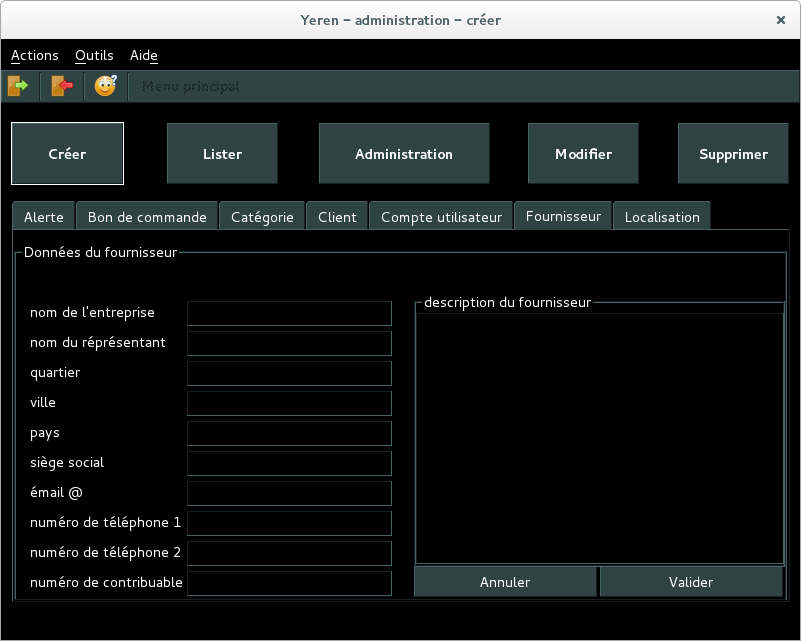
\includegraphics[scale=0.45]{images/compte-fournisseur-creer.png}
	\caption{L'interface graphique pour cr\'eer un
			nouveau compte fournisseur.}
	\label{fig:admin-comptes-fournisseurs-creer}
\end{figure}

La figure~\ref{fig:admin-comptes-fournisseurs-creer} illustre
l'interface graphique de \yeren pour cr\'eer un nouveau
compte fournisseur.

\procparagraph{Proc\'edure pour cr\'eer un compte fournisseur}
\begin{enumerate}[1)]
	\item \`A partir de l'interface graphique de l'acceuil de
		l'administration (voir figure~\ref{fig:fenetre-administrateur}),
		on clique sur l'onglet intitul\'e \textbf{op\'erations}. 
		
	\item Choisir '\textbf{cr\'eer}' dans le '\emph{combo box
		op\'erations}'.
		
	\item Choisir '\textbf{un compte fournisseur}' dans
		le '\emph{combo box objets}'. Vous \^etes automatiquement
		conduit \`a la fen\^etre illustr\'ee par la
		figure~\ref{fig:admin-comptes-fournisseurs-creer}.
		
	\item Saisissez les informations requises dans les champs de texte
		suivants:
		\begin{enumerate}[1)]
			\item nom de l'entreprise
			\item nom du r\'epr\'esentant \optionel
			\item quartier \optionel
			\item ville \optionel
			\item pays \optionel
			\item si\`ege social \optionel
			\item \'email@ \optionel
			\item num\'ero de t\'el\'ephone 1 \optionel
			\item num\'ero de t\'el\'ephone 2 \optionel
			\item num\'ero de contribuable \optionel
			\item description du fournisseur. \optionel			
		\end{enumerate}
		
	\item Cliquer sur le bouton \bouton{Valider} pour
		valider votre travail.		
\end{enumerate}

%%%%%%%%%%%%%%%%%%%%%%%%%%%%%%%%%%%%%%%%%%%%%%%%%%%%%%%%%%%%%%%%%%%%%%%%%%%%%%%%%

\newpage
\nxsubsection{Lister les fournisseurs}
\index{lister les fournisseurs}

\begin{figure}[!htpb]
	\centering
	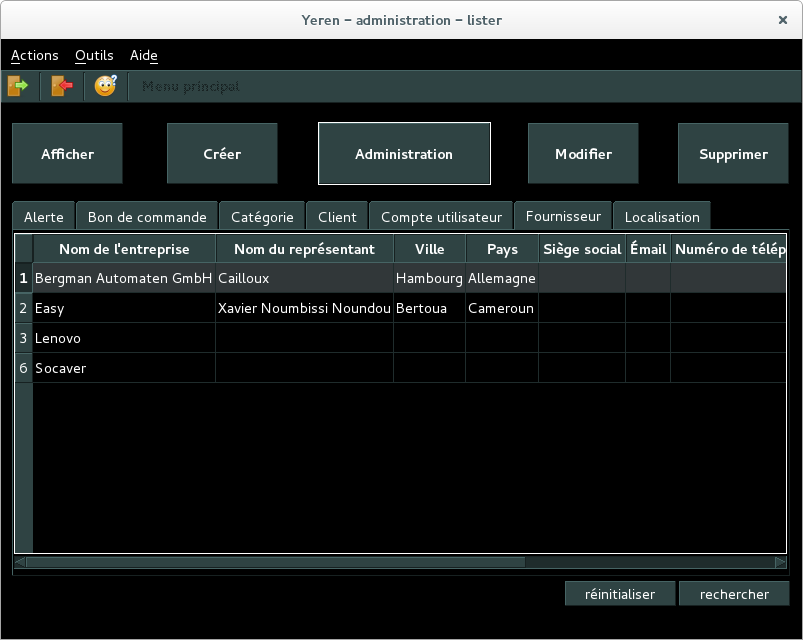
\includegraphics[scale=0.45]{images/compte-fournisseur-lister.png}
	\caption{L'interface graphique pour lister les comptes fournisseurs.}
	\label{fig:admin-comptes-fournisseurs-lister}
\end{figure}

La figure~\ref{fig:admin-comptes-fournisseurs-lister} illustre
l'interface graphique de \yeren qui liste les comptes fournisseurs.

\procparagraph{Proc\'edure pour lister les comptes fournisseurs}
\begin{enumerate}[1)]
	\item \`A partir de l'interface graphique de l'acceuil de
		l'administration (voir figure~\ref{fig:fenetre-administrateur}),
		on clique sur l'onglet intitul\'e \textbf{op\'erations}. 
		
	\item Choisir '\textbf{lister}' dans le '\emph{combo box
		op\'erations}'.
		
	\item Choisir '\textbf{un compte fournisseur}' dans
		le '\emph{combo box objets}'. Vous \^etes automatiquement
		conduit \`a la fen\^etre qui liste les comptes fournisseurs
		(figure~\ref{fig:admin-comptes-fournisseurs-lister}).
\end{enumerate}

%%%%%%%%%%%%%%%%%%%%%%%%%%%%%%%%%%%%%%%%%%%%%%%%%%%%%%%%%%%%%%%%%%%%%%%%%%%%%%%%%

\newpage
\nxsubsection{Modifier les d\'etails d'un fournisseur}
\index{modifier les d\'etails d'un fournisseur}

\begin{figure}[!htpb]
	\centering
	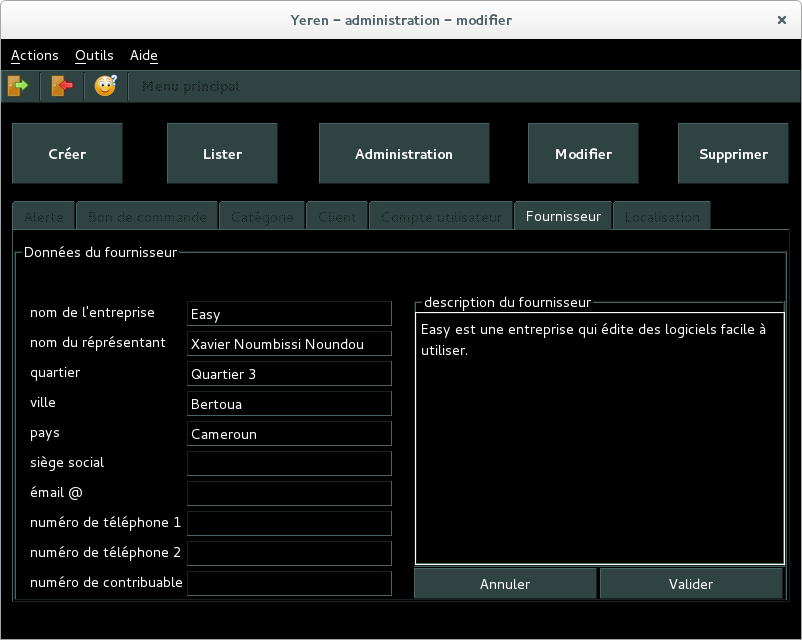
\includegraphics[scale=0.45]{images/compte-fournisseur-modifier.png}
	\caption{L'interface graphique pour modifier les
			d\'etails d'un compte fournisseur.}
	\label{fig:admin-comptes-fournisseurs-modifier}
\end{figure}

La figure~\ref{fig:admin-comptes-fournisseurs-modifier} illustre
l'interface graphique de \yeren pour modifier les
d\'etails d'un compte fournisseur.

\procparagraph{Proc\'edure pour modifier les d\'etails d'un compte fournisseur}
\begin{enumerate}[1)]
	\item \`A partir de l'interface graphique de l'acceuil de
		l'administration (voir figure~\ref{fig:fenetre-administrateur}),
		on clique sur l'onglet intitul\'e \textbf{op\'erations}. 
		
	\item Choisir '\textbf{lister}' dans le '\emph{combo box
		op\'erations}'.
		
	\item Choisir '\textbf{un compte fournisseur}' dans le '\emph{combo box
		sujets}'. Vous \^etes automatiquement conduit \`a la fen\^etre
		illustr\'ee par la figure~\ref{fig:admin-comptes-fournisseurs-lister}.
		
	\item S\'electionner le compte fournisseur dont vous souhaitez
		modifier les d\'etails dans la liste des comptes fournisseurs
		affich\'ee.
		
	\item Cliquer sur le bouton \bouton{Modifier}. Les d\'etails
		du compte fournisseur sont affich\'es dans une nouvelle fen\^etre.
		
	\item Faites les modifications que vous souhaitez.
		
	\item Cliquer sur le bouton \bouton{valider} pour valider
		les modifications faites.
\end{enumerate}

%%%%%%%%%%%%%%%%%%%%%%%%%%%%%%%%%%%%%%%%%%%%%%%%%%%%%%%%%%%%%%%%%%%%%%%%%%%%%%%%%

\newpage
\nxsubsection{Supprimer un compte fournisseur}
\index{supprimer un compte fournisseur}

\begin{figure}[!htpb]
	\centering
	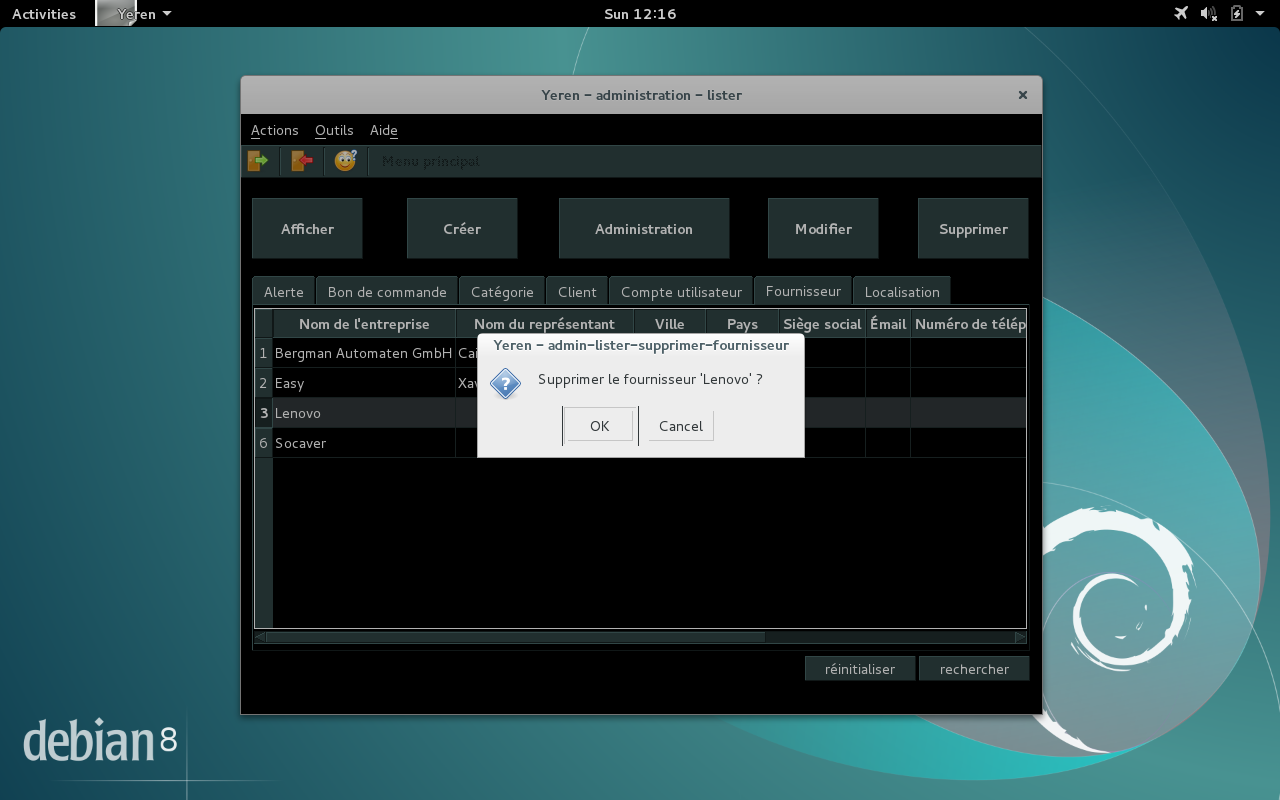
\includegraphics[scale=0.39]{images/compte-fournisseur-supprimer.png}
	\caption{L'interface graphique pour supprimer un fournisseur.}
	\label{fig:admin-comptes-fournisseurs-supprimer}
\end{figure}

La figure~\ref{fig:admin-comptes-fournisseurs-supprimer}
illustre l'interface graphique de \yeren pour supprimer
un compte fournisseur.

\procparagraph{Proc\'edure pour supprimer un compte fournisseur}
\begin{enumerate}[1)]
	\item \`A partir de l'interface graphique de l'acceuil de
		l'administration (voir figure~\ref{fig:fenetre-administrateur}),
		on clique sur l'onglet intitul\'e \textbf{op\'erations}. 
		
	\item Choisir '\textbf{supprimer}' dans le '\emph{combo box
		op\'erations}'.
		
	\item Choisir '\textbf{un compte fournisseur}' dans le
		'\emph{combo box objets}'. Vous \^etes automatiquement
		conduit \`a la fen\^etre illustr\'ee par la
		figure~\ref{fig:admin-comptes-fournisseurs-lister}.
		
	\item S\'electionner le compte fournisseur \`a supprimer
		dans la liste des comptes fournisseurs affich\'ee.
		
	\item Cliquer sur le bouton \bouton{Supprimer}. La question
		est ensuite pos\'ee si vous confirmer votre choix.
		Cliquer sur le \bouton{OK} pour confirmer votre choix.
\end{enumerate}
